
Ce premier chapitre est consacr\'e \`a un \'etat des
lieux des probl\`emes concrets auxquels nous avons
\'et\'e confront\'es et qui ont motiv\'e ce travail du point de
vue de \textsf{Norsys}. L'arriv\'ee des technologies dites nouvelles,
c'est \`a dire le d\'eveloppement de logiciels r\'epartis \`a
destination de clients l\'egers, avait pour but de pallier au probl\`eme de
maintenance et d'\'evolutivit\'e des syst\`emes client-serveurs ou
sites centraux. Ces technologies --- langages orient\'e-objets,
intergiciels, r\'eseaux ouverts, ... ---  ont induit une modification du processus de
d\'eveloppement. Cette \'evolution s'est faite progressivement au
fil des nouveaux projets, avec
l'int\'egration de nouvelles m\'ethodes de conception dirig\'ees
par les mod\`eles \textsf{UML} et de nouvelles pratiques  inspir\'ees
des techniques des logiciels libres et de 
l'\emph{eXtreme Programming}. Le constat que l'on peut faire
aujourd'hui et qui sera d\'evelopp\'e dans ce chapitre est que, si
la phase de d\'eveloppement et dans l'ensemble les aspects
technologiques sont bien ma\^{\i}tris\'es, la conception des
syst\`emes, leur articulation avec l'analyse des besoins du client et
surtout la qualit\'e et la fiabilit\'e du produit fini posent encore
de nombreux probl\`emes. Ces probl\`emes nous semblent provenir d'un manque de
maturit\'e du processus, de compr\'ehension globale de
l'architecture des syst\`emes et de formalisation du processus de
validation et de v\'erification des d\'eveloppements. 

Nous commencerons ce chapitre par une pr\'esentation du processus de
d\'eveloppement qui nous permettra d'exposer les pratiques actuelles, les outils et  les
m\'ethodes. Cette pr\'esentation nous permettra par ailleurs de
pr\'esenter nos contributions pratiques dans l'am\'elioration du
suivi et de la qualit\'e du processus de d\'eveloppement de ce typ e
d'application. Cette premi\`ere section sera suivie d'une analyse
critique de ce processus et d'une premi\`ere exposition des solutions
envisageables qui nous permettra de mettre l'accent sur les besoins de
formalisation et de v\'erification d'architectures.

\section{\'Etat de la pratique}

\textsf{Norsys} est une soci\'et\'e de services et comme telle est
amen\'ee \`a r\'ealiser des logiciels \`a fa\c{c}on pour un grand
nombre de clients poss\'edant chacun des m\'etiers
diff\'erents. Toutefois, tous les d\'eveloppements r\'ealis\'es
depuis quelques ann\'ees dans le domaine des \og nouvelles
technologies\fg{} poss\`edent nombres de caract\'eristiques communes :
\begin{itemize}
  \item le langage support est \textsf{Java} ;
  \item l'infrastructure technique est bas\'ee sur \textsf{J2EE}\cite{j2eespec}, la
    sp\'ecification orient\'e-composants de \textsf{Sun} pour les
    syst\`emes d'information d'entreprises ;
  \item les phases de recueil des exigences, d'analyse et de conception
    utilisent une mod\'elisation \`a base de diagrammes \textsf{UML}
    compl\'et\'ee de nombreux documents textuels ;
  \item le processus de d\'eveloppement est proche d'un processus de
    type \textsf{RUP} --- \emph{Rational Unified Process} --- avec des points
    d'adaptations sp\'ecifiques et des all\'egements par rapport aux
    pr\'econisations du mod\`ele ;
  \item l'architecture logicielle est structur\'ee en \emph{couches},
    depuis la pr\'esentation jusqu'\`a la persistance des
    donn\'ees. Les services transversaux --- authentification,
    habilitations, contexte transactionnel, r\'epartition de charges,
    ... --- sont assur\'es par l'infrastructure \textsf{J2EE} ou
    d\'evelopp\'es de mani\`ere ad-hoc ;
  \item les syst\`emes d\'evelopp\'es ont g\'en\'eralement \`a
    s'int\'egrer dans un existant complexe, m\'elange d'applications
    client-serveurs, de bases de donn\'ees, de
    moniteurs transactionnels et de syst\`emes centralis\'es en
    \textsf{COBOL}.
\end{itemize}

\subsection{Infrastructure technique}
\label{sec:infr-techn}
La cible technique est constitu\'ee de syst\`emes r\'epartis
g\'en\'eralement redondants h\'eberg\'es sur des fermes de
serveurs. La figure \ref{fig-infra-technique} repr\'esente une
architecture technique type sur laquelle sont d\'eploy\'ees les
applications produites. Il s'agit l\`a bien \'evidemment d'une configuration id\'eale qui
peut \^etre adapt\'ee en fonction des contraintes de co\^uts, de
performances ou de s\'ecurit\'e du projet. 

\begin{figure}[htbp]
    \centering
    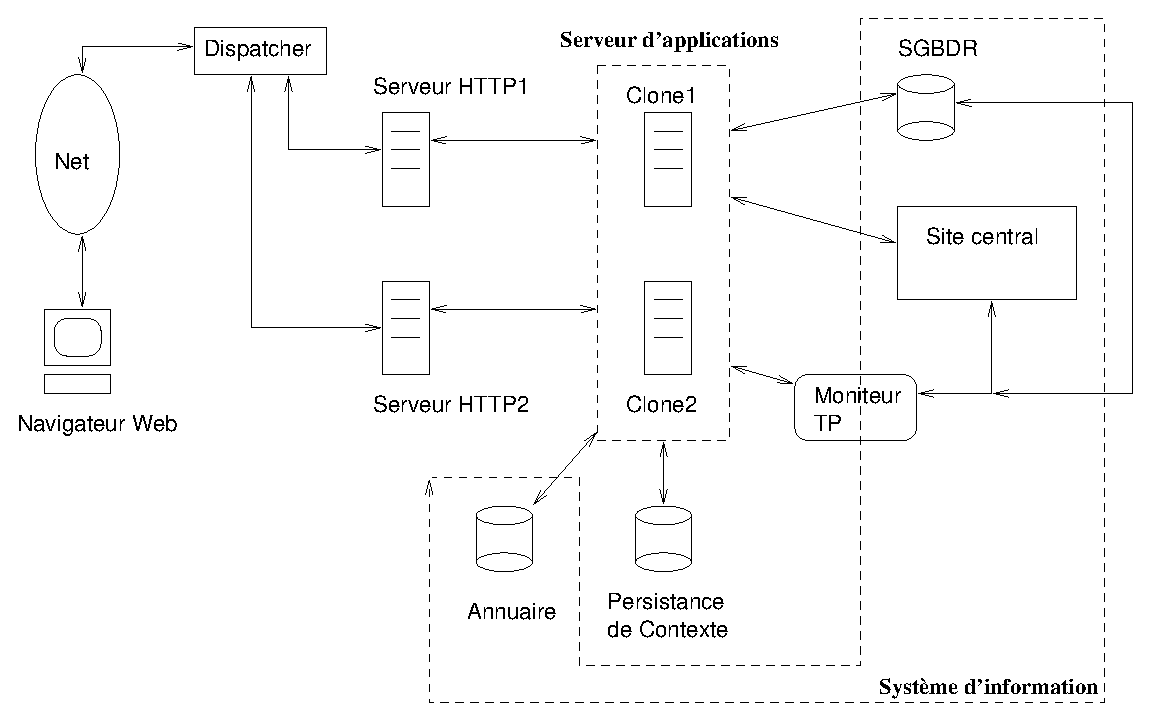
\epsfig{width=.9\textwidth,file=figures/fig-infra-technique.eps}
    \caption{Architecture technique}
    \label{fig-infra-technique}
\end{figure}

La communication avec le client est g\'er\'ee par un ou plusieurs
serveurs HTTP avec un r\'epartiteur de charge permettant de minimiser
temps de r\'eponses et trafic r\'eseau. Le serveur \textsf{HTTP}
communique avec le \emph{serveur d'applications} g\'en\'eralement au
travers d'un protocole ad-hoc, serveur qui peut \^etre clon\'e de
sorte que l\`a aussi, la charge soit r\'epartie sur plusieurs
machines et la tol\'erance aux pannes soit am\'elior\'ee.  Le
contexte, c'est \`a dire l'ensemble des informations relatives \`a
une session, est persistant selon un m\'ecanisme
propre au serveur
d'applications choisi. Les besoins d'authentification des clients,
qu'ils soient r\'ealis\'es par mots de passe ou par une
infrastructure \`a cl\'es publiques (\textsf{PKI}), sont
le plus souvent g\'er\'es par un annuaire d'entreprise de type
\textsf{LDAP}. Il en va de m\^eme pour l'habilitation des
utilisateurs, c'est \`a dire pour la d\'efinition de leurs droits
d'acc\`es sur les fonctions du syst\`eme. Notons que
l'authentification se fait g\'en\'eralement au niveau des serveurs
HTTP tandis que l'habilitation se fait dans le serveur d'applications. 

Le serveur d'applications contient l'ensemble de la logique  de
l'application (voir ci-dessous) et a la charge de communiquer au
travers de connecteurs idoines avec le reste du syst\`eme
d'information : bases de donn\'ees relationnelles, sites centraux,
moniteurs transactionnels. L'architecture \textsf{J2EE} pr\'evoit, au travers
des connecteurs \textsf{JCA}, la possibilit\'e de relier un tel
syst\`eme \`a n'importe quel autre  en maintenant des
propri\'et\'es transactionnelles. Pour une pr\'esentation
g\'en\'erale de l'architecture de la plateforme \textsf{J2EE}, voir
la section \ref{sec:j2ee} du chapitre \ref{chap-etatart}.

\subsection{Architecture logicielle}
\label{sec:arch-logic}
L'architecture logicielle utilis\'ee est une architecture en couches 
qui reprend un certain nombre de \og bonnes pratiques\fg{} d\'esormais
courantes dans le domaine. Elle s'inspire  de
\emph{patrons de conceptions}\cite{core-j2ee-patterns,gof} usuels, tels que le patron
\emph{Mod\`ele-Vue-Contr\^oleur} popularis\'e par le framework
\textsf{Struts} pour la gestion des interactions avec le client, ou
le patron \emph{Recherche de Services}  --- 
\emph{Service Locator} --- pour la localisation d'interfaces
m\'etiers offertes par les \textsf{EJB}. La figure
\ref{fig-archi-couche} reprend les diff\'erents \'el\'ements de
mani\`ere synth\'etique. 

\begin{figure}[htbp]
    \centering
    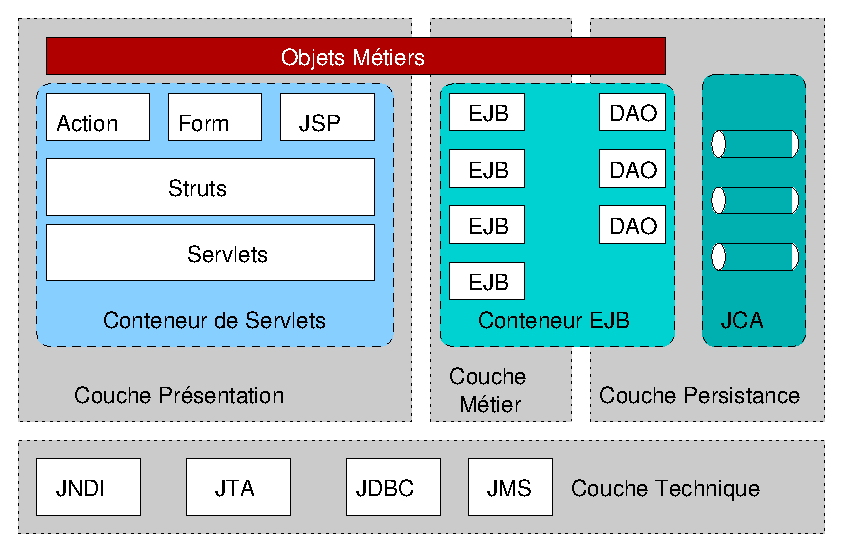
\epsfig{width=.9\textwidth,file=figures/fig-archi-couche.eps}
    \caption{Architecture logicielle}
    \label{fig-archi-couche}
\end{figure}

La \emph{couche pr\'esentation} s'appuie sur des \emph{servlets}
encapsul\'ees dans un conteneur, qui
permettent de d\'evelopper des contenus dynamiques en
\textsf{Java} en s'abstrayant d'un certain nombre de d\'etails
techniques tels que la gestion de la transformation des param\`etres
--- \emph{marshalling} --- depuis ou vers le protocole \textsf{HTTP},
la gestion du contexte de session et du contexte applicatif et surtout
la communication par appels de m\'ethodes distants avec la couche
m\'etier, c'est \`a dire les
\textsf{EJB}. \textsf{Struts} fournit
un canevas pour g\'erer les interactions avec le client et sur cette
base sont d\'evelopp\'es des \emph{actions}, des \emph{formulaires}
--- \emph{forms} --- et des \textsf{JSP} --- \emph{Java Server Pages}
--- repr\'esentant respectivement la partie contr\^ole, mod\`ele
et vue du patron \textsf{MVC}. 

La \emph{couche m\'etier} contient les \emph{Enterprise Java Beans},
un ensemble de services m\'etiers utilis\'es par la couche
pr\'esentation en fonction des besoins de l'application. Ces
\textsf{EJB} sont le plus souvent de type \emph{Session sans \'etat}
et le traitement de l'acc\`es aux donn\'ees est d\'el\'egu\'e
\`a des objets sp\'ecialis\'es appel\'es \emph{Data Access
  Objects} ou \textsf{DAO}, plut\^ot que laiss\'e \`a la
discr\'etion du conteneur et d'\textsf{EJB} \emph{Entit\'es}. 

La couche persistance est souvent la plus technique et la plus
d\'elicate. Dans l'id\'eal, elle r\'ealise une simple projection du
mod\`ele de classes des objets m\'etiers depuis ou vers un syst\`eme de base
de donn\'ees quelconque, ce qui peut \^etre fait de mani\`ere
automatis\'ee en s'appuyant sur un framework tel que les EJB
\emph{Entit\'es} ou \textsf{Hibernate}. Dans la pratique, compte tenu du fait
que les sch\'emas de table sont g\'en\'eralement pr\'eexistants
aux applications d\'evelopp\'ees, que les canevas de projection
objet-relationnel automatis\'es ont du mal \`a optimiser
correctement les transactions et les requ\^etes et que l'on a pas
uniquement affaire \`a des syst\`emes relationnels mais aussi
\`a des applications l\'egataires, \`a des transactions stock\'ees
\textsf{COBOL} ou encore \`a des couches de moniteurs transactionnels
propri\'etaires, cette gestion est le
plus souvent d\'evelopp\'ee de mani\`ere ad-hoc. 

La couche transversale \emph{objets m\'etiers} contient l'ensemble
des objets du domaine applicatif, autrement dit l'instantiation du
diagramme de classes des donn\'ees manipul\'ees par
l'application. Ces objets sont utilis\'es par toutes les couches, l'utilisation
d'objets dans les interactions entre couches permettant par ailleurs de
r\'eduire le nombre d'appels de m\'ethodes r\'ealis\'es et donc
d'accro\^{\i}tre les performances du syst\`eme. 

La couche technique, enfin, comprend un certain nombre de services sur
lesquels s'appuient les diff\'erents composants du syst\`eme :
\begin{itemize}
  \item service de nommage --- \emph{Java Naming and Directory
  Interface} ;
\item service de transaction --- \emph{Java Transaction API} ;
\item service d'acc\`es aux donn\'ees --- \emph{Java DataBase
    Connectivity} ;
\item service de messagerie asynchrone --- \emph{Java Message Service}.
\end{itemize}

\subsection{Processus de d\'eveloppement}

Le processus de d\'eveloppement utilis\'e est largement inspir\'e
du \emph{Rational Unified Process} ou \textsf{RUP}, m\^atin\'e d'une
bonne dose de pragmatisme et d'un zeste d'\emph{eXtreme
  Programming}. Nous renvoyons aux travaux r\'ealis\'es au sein de
l'entreprise par E.\textsc{Renaux}\cite{these-manu} pour une analyse
plus pouss\'ee de ce processus et de ses d\'efauts. 

Il s'agit l\`a d'un principe th\'eorique qui dans la  pratique
recouvre un d\'ecoupage plus \og traditionnel\fg{}  en activit\'es et
en lots :
\begin{itemize}
  \item les phases d'\emph{expression des besoins} et d'\emph{analyse} se confondent dans une
  m\^eme phase. Elles produisent un cahier des charges, des
  diagrammes de cas d'utilisation, des sc\'enarios  et des r\`egles
  m\'etiers ;
\item la \emph{conception} produit les
  diagrammes de classes et \'eventuellement d'\'etats-transitions
  associ\'es, ainsi que les sch\'emas de donn\'ees ;
\item le \emph{d\'eveloppement} r\'ealise effectivement
  l'application \`a partir des documents de conception ;
\item la phase de test ou phase de \emph{recette} valide l'application
  produite par rapport aux besoins initiaux.
\end{itemize}
Les it\'erations et incr\'ements  ont une granularit\'e beaucoup
plus grande que dans les pr\'econisations des m\'ethodes cit\'ees,
un probl\`eme  important dont on verra par la suite qu'il
d\'ecoule de carences dans la mod\'elisation de l'architecture
globale de l'application.

Le processus de d\'eveloppement s'appuie par ailleurs sur une analyse
d'\emph{urbanisation} du syst\`eme d'informations qui permet de
d\'ecouper globalement les processus m\'etiers en diff\'erents
\emph{quartiers} et \emph{blocs} reproduisant au niveau informatique
l'organisation du client.  Le processus tel que nous le pr\'esentons
ici doit \^etre compris comme une synth\`ese d'un ensemble de
pratiques dans diff\'erents contextes.  

\subsection{M\'ethodologie d'analyse \& conception}

La m\'ethodologie articule la conception en \emph{couches} et le
r\'esultat du processus d'analyse en \emph{vues}. Les diff\'erentes
couches recens\'ees sont:
\begin{itemize}
\item la couche \emph{Pr\'esentation} qui contient essentiellement les
\'el\'ements r\'egissant les interactions avec l'utilisateur :
description de l'interface graphique, r\`egles de navigation entre
\'ecrans ;
\item la couche \emph{Dynamique applicative} qui contient les processus de
l'application proprement dite, c'est \`a dire essentiellement les
actions \textsf{Struts} ;
\item la couche \emph{M\'etier} qui d\'efinit et contient les services
m\'etiers et les objets associ\'es ;
\item la couche \emph{Persistance} qui d\'ecrit les r\`egles d'interaction
entre objets-m\'etiers et syst\`eme de stockage.
\end{itemize}

Le processus d'analyse et de conception est d\'ecoup\'e en vues qui
sont chacune repr\'esent\'ees par diff\'erents mod\`eles \textsf{UML} et
\'el\'ements de documentation. Ces diff\'erentes vues sont:
\begin{itemize}
\item la \textbf{vue utilisateur} qui d\'ecrit les besoins de l'utilisateurs en
termes g\'en\'eraux ;
\item la \textbf{vue processus} qui mod\'elise chaque processus d'interaction
entre un utilisateur et le syst\`eme ;
\item la \textbf{vue composant} qui identifie les composants du syst\`eme,
leur fonctionnement et leur interaction avec d'autres composants ;
\item la \textbf{vue persistance} qui d\'ecrit les r\`egles de projection
entre objets-m\'etiers et syst\`eme de stockage persistant.
\end{itemize}

Nous d\'ecrivons succintement
chacune des vues dans les sections ci-dessous en proposant
syst\'ematiquement une synth\`ese sous la forme d'un
\emph{m\'eta-mod\`ele} \textsf{UML} de chaque vue.

\subsubsection{Vue utilisateur}

Les besoins utilsateurs sont d\'ecrits sous la forme de diagrammes de cas
d'utilisation et de diagrammes de classes. Un m\'eta-mod\`ele de
cette vue utilisateur est donn\'e ci-dessous (partie sup\'erieure de la
figure \ref{fig-vue-utilisateur}).

\begin{figure}[htbp]
    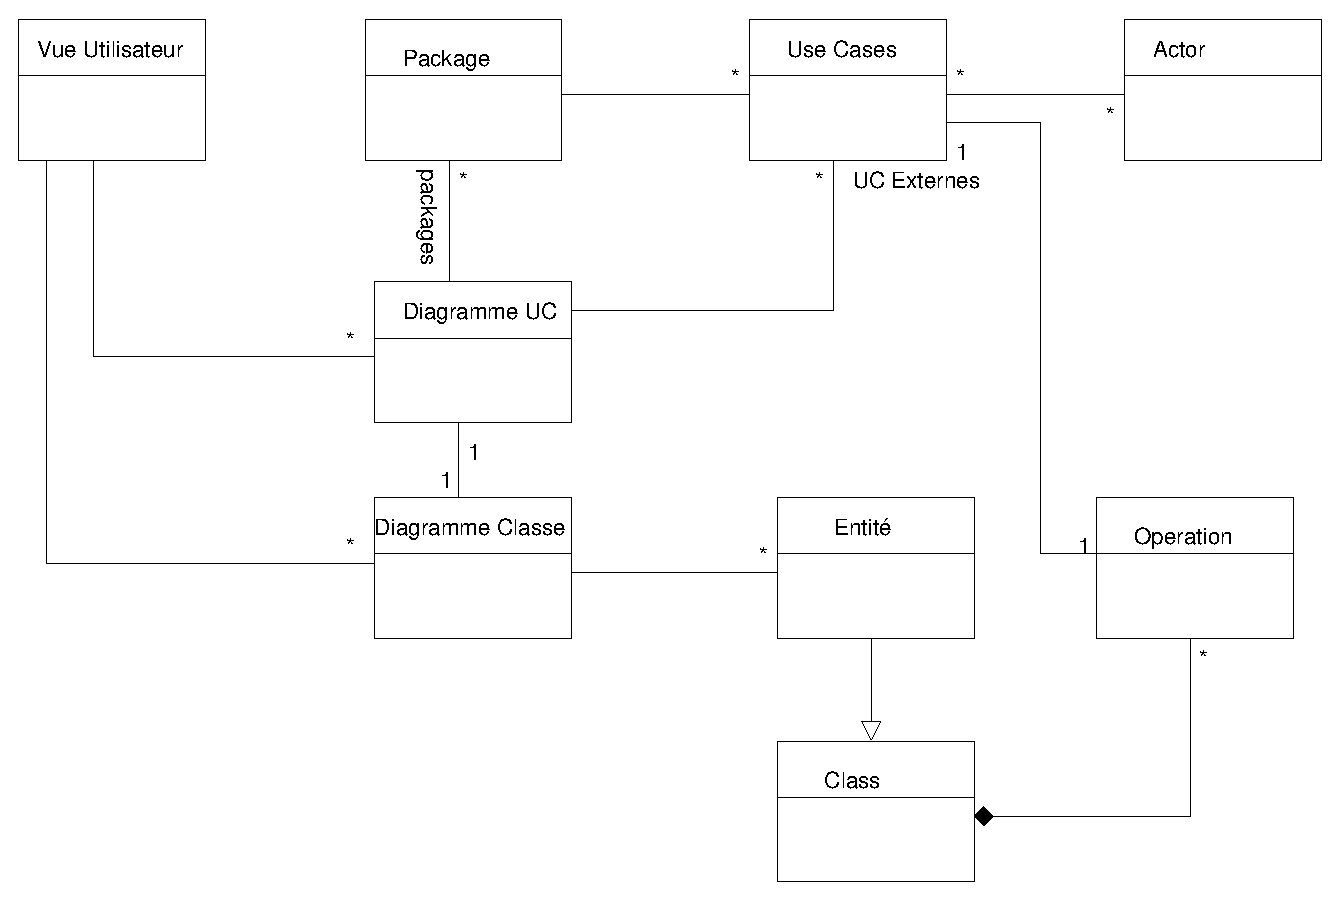
\epsfig{width=.60\textwidth,file=figures/vue-util-mm.eps}\hfill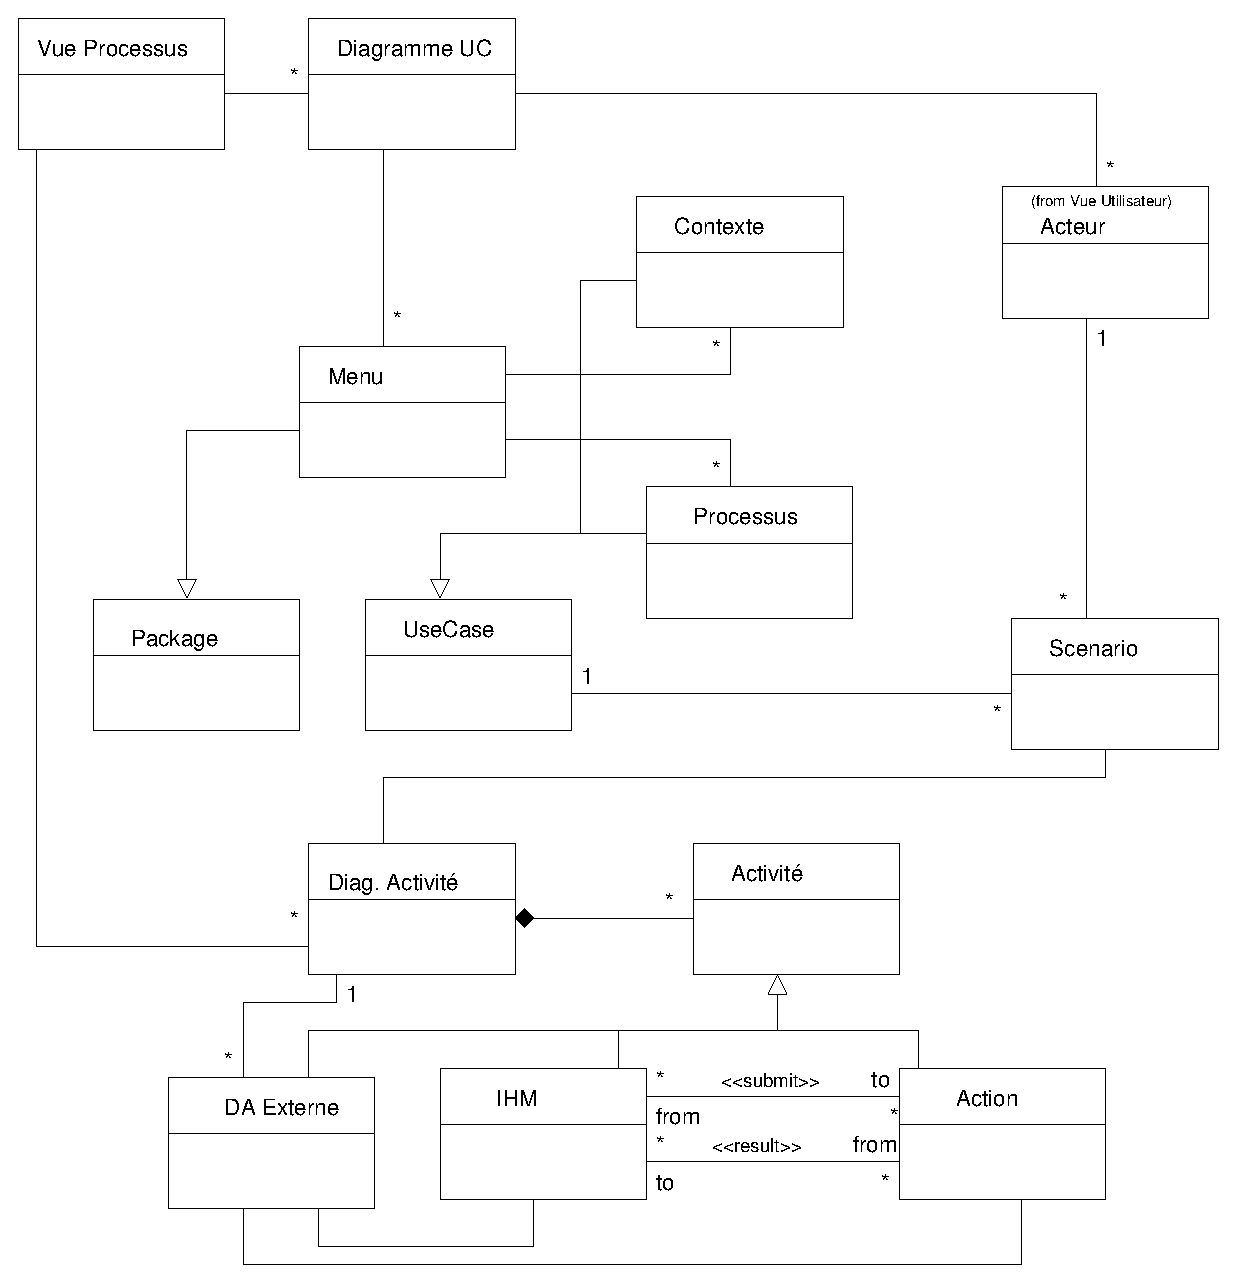
\epsfig{width=.60\textwidth,file=figures/vue-proc-mm.eps}
\centering
    \caption{Vues utilisateurs \& m\'etiers}
    \label{fig-vue-utilisateur}
\end{figure}

Dans cette vue, on exprime les besoins de l'utilisateur, d\'efinit
le p\'erim\`etre du syst\`eme, les interactions avec les
diff\'erents r\^oles de l'utilisateur. Cette vue permet de
d\'egager des \textbf{entit\'es fonctionnelles} (domaines)
repr\'esent\'ees dans le m\'eta-mod\`ele par une classe dont les
attributs sont d\'efinis par les cas d'utilisation.

\subsubsection{Vue Processus}

Cette vue, \`a partir des besoins utilisateurs exprim\'ees
pr\'ec\'edemment, va d\'efinir pr\'ecis\'ement les interactions
existant entre les diff\'erents r\^oles (acteurs) intervenant dans
l'application et  le syt\`eme. Ces interactions sont
repr\'esent\'ees dans une diagramme de cas d'utilisation, chaque cas
d'utilisation se trouvant par la suite associ\'e \`a un ou plusieurs
diagrammes d'activit\'e. Les regroupements de cas d'utilisation
repr\'esentent en fait des menus/actions acccessibles par
diff\'erents r\^oles du syst\`eme et leur organisation.

Cette vue permet en particulier d'indentifier et de caract\'eriser
les objets \textsf{IHM} utilis\'es (types d'\'el\'ements d'interfaces,
ordres de navigation, accessibilit\'e) et de d\'efinir les processus m\'etiers,
c'est \`a dire de documenter les algorithmes relatifs \`a chaque
\verb|Action| : quelles sont les \'el\'ements de donn\'ees de
l'\textsf{IHM} qui sont transmis et quels sont les r\'esultats ?

\subsubsection{Vue Composants}

La vue \og composants\fg{} d\'etaille:
\begin{itemize}
\item les \'el\'ements d'\textsf{IHM}, plus
particuli\`erement du point de vue de la couche dynamique
applicative, c'est \`a dire du \emph{serveur d'application} dans
l'architecture choisie ;
\item les services m\'etiers, c'est \`a dire les objets et leurs
interfaces permettant de r\'ealiser les fonctions demand\'ees par
l'utilisateur.
\end{itemize}

\begin{figure}[htbp]
    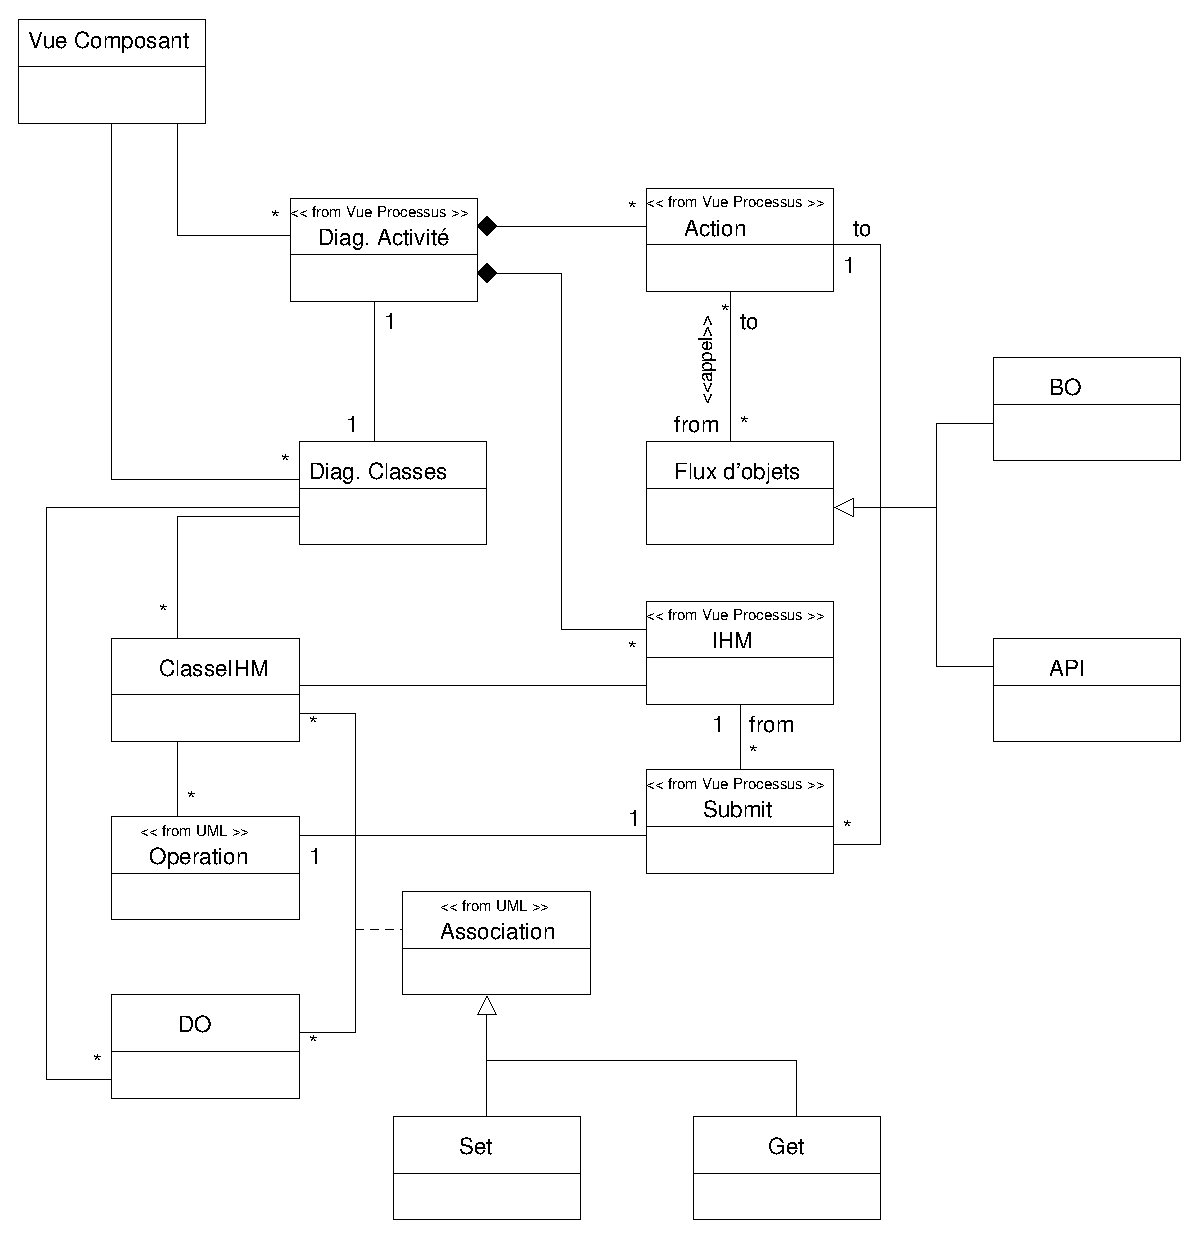
\epsfig{width=.60\textwidth,file=figures/vue-comp-mm.eps}\hfill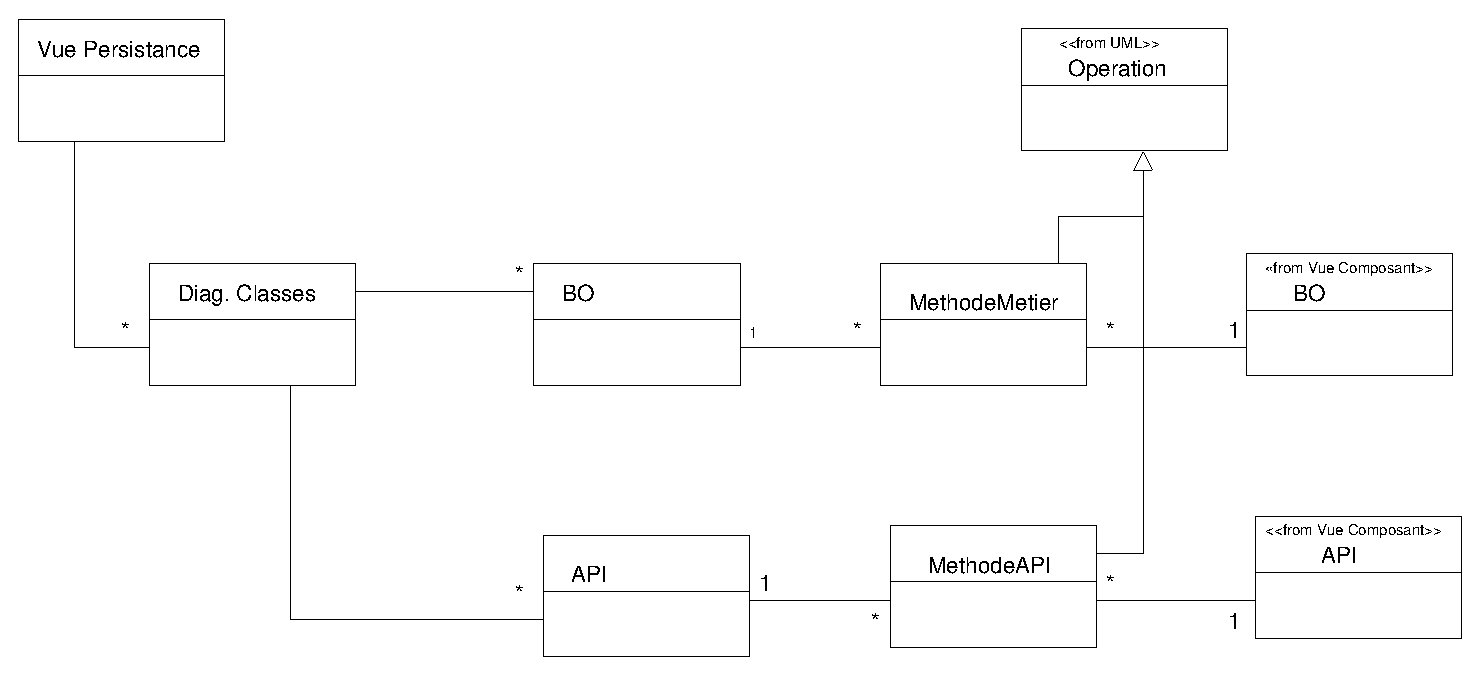
\epsfig{width=.60\textwidth,file=figures/vue-pers-mm.eps}
\centering   
    \caption{Vue composants m\'etiers \& persistance}
    \label{fig-vue-composant}
\end{figure}

Le diagramme d'activit\'e issu de la phase pr\'ec\'edente est
enrichi par des informations suppl\'ementaires sur les \'el\'ements
concrets de r\'ealisation des classes \verb|IHM|  (maquette HTML, page
JSP, attributs) et des \'el\'ements \verb|Flux d'objet|. Ces flux
d'objets correspondent \`a des invocations de services m\'etiers
(BO) ou d'\'el\'ements de l'infrastructure logicielle sous-jacente
(API). \`A chaque transition d\'eclench\'ee par une activit\'e
d'IHM correspond une m\'ethode dans la classe d'IHM correspondante,
m\'ethode qui sera document\'ee en d\'ecrivant les contr\^oles
effectu\'es sur les attributs de l'objet.

\subsubsection{Vue M\'etier/persistance}

Cette derni\`ere vue d\'efinit plus pr\'ecis\`ement les objets
m\'etiers et la mani\`ere dont ces objets sont stock\'es et
correspondent \`a des donn\'ees pr\'esentes dans des applicationss
patrimoniales (sites centraux), des SGBD ou toute autre forme de
projection. Comme indiqu\'e dans le paragraphe pr\'ec\'edent,
les objets BO et API ont pour fonction de faire le lien entre les
services vus du point de vue de l'application et les donn\'ees et
couches techniques.  Des r\`egles d'acc\`es aux
donn\'ees persistantes sont par ailleurs d\'efinies \`a ce stade mais nous avons
choisi de ne pas les analyser dans ce document. Nous  consid\'erons
en effet  qu'il s'agit de probl\`emes de l'ordre de l'implantation et des choix
technologiques r\'ealis\'es qui ne doivent pas avoir d'impact sur
les \textbf{fonctionnalit\'es}  de l'application.

\subsection{Infrastructure de d\'eveloppement}

Les d\'eveloppements s'appuient sur un certains nombres d'outils et
de pratiques ayant pour objectif d'accro\^{\i}tre la qualit\'e et la
fiabilit\'e du r\'esultat final. D'une part, ils s'appuient sur une
d\'emarche globale d'\emph{ing\'eni\'erie dirig\'ee par les
  mod\`eles} permettant de tirer partie de l'existence de mod\`eles
de conception et de lib\'erer le d\'eveloppeur des contraintes
techniques induites par la plateforme. Concr\`etement, cela signifie
qu'\`a partir des diagrammes de classes des objets m\'etiers, on utilise des outils de g\'en\'eration de code pour
produire automatiquement les \'el\'ements n\'ecessaires \`a
l'infrastructure technique : interfaces distantes et fabriques dans le
cas des \textsf{EJB}, fichiers de configurations \textsf{XML} pour la
persistance des donn\'ees et la couche pr\'esentation, formulaires
\textsf{Struts}.

D'autre part, un processus d'\emph{int\'egration continue} pilot\'e
par \textsf{Maven} et bas\'e
sur un \emph{syst\`eme de gestion de versions} permet d'automatiser
la construction des d\'elivrables de l'applications --- paquetages,
archives, descripteurs de d\'eploiement ---- et surtout de produire
\`a intervalles r\'eguliers une photographie de l'ensemble de
l'application, de sa documentation et une batterie de
v\'erifications statiques et dynamiques. Ce principe est r\'esum\'e
dans la figure \ref{fig-develmvc} et reprend la forme d'un patron
\textsf{MVC} dans lequel les vues sont les diff\'erentes phases ou
acteurs du processus de d\'eveloppement, le contr\^oleur est le
moteur d'int\'egration continue et le mod\`ele est le syst\`eme de
gestion de configurations.  

\begin{figure}[htbp]
    \centering
    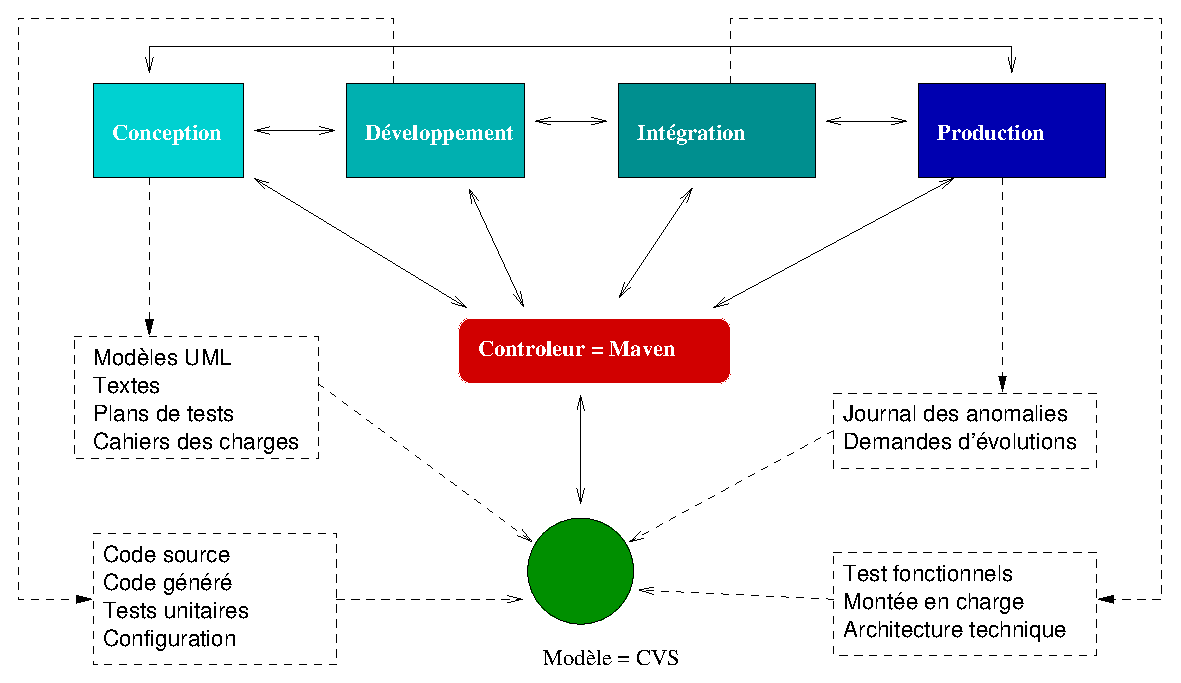
\epsfig{width=.8\textwidth,file=figures/fig-develmvc.eps}
    \caption{Mod\`ele de processus de d\'eveloppement}
    \label{fig-develmvc}
\end{figure}

Les v\'erifications r\'ealis\'ees par le contr\^oleur \`a partir
du code source sont les suivantes :
\begin{itemize}
  \item v\'erifications des r\`egles syntaxiques de codage : nommage
  des entit\'es dans le code, indentation et formatage, ... ;
\item v\'erifications de r\`egles --- simples --- de s\'emantique :
  code mort, variables inutilis\'ees et d\'eclarations incorrectes,
  ... ;
\item calculs de m\'etriques par paquetage telles que le degr\'e
  d'abstraction/concr\'etion, le taux de couplage, le degr\'e de
  complexit\'e, ... ;
\item v\'erification des r\`egles d'acc\`es architecturales entre
  classes et paquetages permettant de v\'erifier le respect par les
  d\'eveloppeurs de l'architecture globale  du syst\`eme ;
\item ex\'ecution des tests unitaires et calcul de la couverture de
  code --- instructions et branchements --- r\'ealis\'ee.
\end{itemize}

Le d\'eveloppement et la mise en \oe uvre de ces outils a
constitu\'e une part importante  de notre contribution au sein de
l'entreprise et s'est \'etal\'ee sur diff\'erents projets. En l'\'etat actuel des choses, seule la
vue \emph{D\'eveloppement} est r\'eellement op\'erationnelle. Une
partie de l'objectif de cette th\`ese est de faire en sorte que les
autres vues, et plus particuli\`erement les vues \emph{Conception} et
\emph{Int\'egration} soient misent en places par la gestion
automatis\'ee des tests fonctionnels \`a diff\'erents niveaux de
l'architecture et la validation crois\'ee entre mod\`eles et
sources. 

\section{Analyse critique}
\label{sec:analyse-critique}
Apr\`es un rapide tour d'horizon du processus de d\'eveloppement
type d'applications r\'eparties sur architecture \textsf{J2EE} tel
que nous le pratiquons aujourd'hui, cette section est consacr\'ee
\`a une analyse critique dudit processus en partant des probl\`emes
constat\'es concr\`etement lors de la vie des projets et des
\'el\'ements m\'ethodologiques pr\'esent\'es. 

Comme l'a fort bien soulign\'e E.\textsc{Renaux} dans ses travaux
pr\'ec\'edemment cit\'es, un des probl\`emes essentiels auquel
nous sommes confront\'es est le passage de l'\emph{analyse} \`a la
\emph{conception}, c'est \`a dire la transformation d'un sch\'ema de
compr\'ehension g\'en\'eral du processus m\'etier de l'application
en un mod\`ele de conception \`a base de composants. La propositon
\emph{Component Unified Process}\cite{manu-cup-lmo,these-manu} a pour objectif de r\'esoudre ce
probl\`eme en introduisant au plus t\^ot une structuration en
composants des diff\'erentes fonctionnalit\'es de
l'application. Notons que c'est partiellement ce qui est
pr\'econis\'e dans le processus de mod\'elisation que nous avons
d\'etaill\'e ci-dessus. 

Nous nous int\'eressons toutefois \`a un probl\`eme diff\'erent :
il s'agit, rappelons-le, de v\'erifier que ce qui est d\'evelopp\'e
correspond bien \`a ce qui est attendu, pas plus, pas moins. Notre
analyse sera donc sous-tendue par cette probl\'ematique.

\subsection{Complexit\'e}

Les syst\`emes d'information en particulier, et les gros syst\`emes
informatiques en g\'en\'eral, ont toujours \'et\'e complexes mais
cette complexit\'e conceptuelle se trouve aujourd'hui
d\'emultipli\'ee par la complexit\'e des architectures techniques
et applicatives mises en place. L'h\'et\'erog\'en\'eit\'e des
syst\`emes, la r\'epartition des processus, l'omnipr\'esence des
r\'eseaux, rendent la t\^ache du concepteur et du d\'eveloppeur
encore plus complexe. Le \og paradigme \fg{} de programmation
orient\'ee-objet n'a rien r\'esolu, bien au contraire, puisqu'il
exige de distribuer non seulement les processus de traitements
informatiques eux-m\^emes mais aussi les processus m\'etiers. 

Les plateformes de composants n'ont pas beaucoup mieux r\'eussi \`a
simplifier le probl\`eme et ont m\^eme plut\^ot accru la
fragilit\'e des applications en les rendant d\'ependantes de
services techniques. Ces derniers sont  parfois difficiles \`a appr\'ehender et toujours
d\'elicats \`a int\'egrer dans une conception de par la
multiplication des fichiers de configurations divers et des
contraintes de programmation et de conception.
Les ateliers de d\'eveloppement, s'ils permettent d'all\'eger
certaines t\^aches, ne r\'esolvent pas tout. 

\subsection{Coh\'erence des \'el\'ements du d\'eveloppement}

Le processus de d\'eveloppement, \`a partir de l'expression des
besoins, n'est absolument pas incr\'emental ni it\'eratif
mais est bien plus proche d'un mod\`ele en cascade traditionnel : les
phases d'analyse, de conception et de d\'eveloppement s'encha\^{\i}nent
dans un ordre descendant mais sans que l'information ne puisse
remonter la \og cascade\fg{}. Au final, il est fr\'equent que les
documents d'analyse et de conception soient obsol\`etes lors de la
livraison. Au mieux, ils sont \'ecrits \`a posteriori en
fonction du code effectivement livr\'e. 

Ce probl\`eme provient de
l'absence de lien direct et surtout automatis\'e avec la r\'ealisation
concr\`ete du logiciel, autrement dit du d\'ecouplage entre les
mod\`eles et le code. M\^eme dans les domaines o\`u le code est
g\'en\'er\'e \`a partir de mod\`eles, l'information est \`a sens
unique et il difficile d'int\'egrer \`a la fois les
d\'eveloppements manuels et la production automatis\'ee d'une partie
du code. 

Au sein des phases d'analyse et de conception elles-m\^emes, la
coh\'erence entre les mod\`eles et le respect d'un certain nombre de
r\`egles g\'en\'erales ne sont pas syst\'ematiquement
v\'erifi\'es. 

Enfin, nombre de d\'eveloppements sont des red\'eveloppements. On
suppose donc que le travail d'analyse a d\'ej\`a \'et\'e fait et
on en fait l'\'economie. Malheureusement, les processus \'evoluent
aussi et sont rarement ind\'ependants des technologies de leur mise
en \oe uvre. Les documents sur lesquels sont bas\'es des
red\'eveloppements sont donc souvent obsol\`etes, incomplets voire
faux, d'o\`u l'impossibilit\'e de valider les logiciels produits \emph{a
priori} et de mani\`ere m\'ecanique.

\subsection{Interp\'en\'etration des domaines}

Les fonctionnalit\'es de l'application se trouvent
souvent m\'elang\'ees \`a des \'el\'ements r\'eglant la navigation et
l'acc\`es de l'utilisateur \`a ces diff\'erentes fonctions. C'est
particuli\`erement le cas dans les \'el\'ements
d'\textsf{IHM}, qui m\'elangent niveaux de validation et r\`egles de
navigation. Il nous semble qu'il s'agit de probl\`emes strictement orthogonaux :
\begin{itemize}
\item l'application offre la possibilit\'e \`a l'utilisateur de
r\'ealiser certaines op\'erations, ce sont les services
offerts. Leur encha\^{\i}nement, leur structure, leurs besoins, l'algorithmique
sont d\'etaill\'es par les diff\'erents documents d\'ecrivant
les processus et le m\'etier. En particulier, les encha\^{\i}nements
de processus n\'ecessaires ou possibles sont mod\'elis\'es sous la
forme de diagrammes d'activit\'es ou automates d'\'etats finis ;
\item l'\textsf{IHM} est une \emph{traduction} \`a l'usage des op\'erateurs humains
interagissant avec le syst\`eme du comportement attendu du
syst\`eme. En particulier, les encha\^{\i}nements impos\'es et les
actions activ\'ees et inactiv\'ees du syst\`eme en fonction de
l'\'etat de l'activit\'e se trouvent r\'ealis\'ees graphiquement
par des modifications d'\'ecran et d'attributs des \'el\'ements
composant l'\textsf{IHM}.
\end{itemize}

On retrouve le m\^eme probl\`eme dans la couche
composants/persistance. Le probl\`eme de la persistance des objets
m\'etiers se trouve trait\'e au m\^eme niveau que celui de leur
d\'efinition et de leur manipulation. Des objets purement
m\'ecaniques  tels que les \emph{objets donn\'ees} se trouvent
pr\'esents dans la mod\'elisation alors m\^eme qu'ils sont
automatiquement g\'en\'er\'es par des r\`egles de projection. Enfin, la structure des tables relationnelles se trouve reproduite,
avec tous les probl\`emes que cela comporte, dans le mod\`ele qui de
facto perd ainsi sa structure objet.

\subsection{Formalisation}

Les mod\`eles d'analyse et de conception ne sont pas tels
quels v\'erifiables automatiquement. Leur coh\'erence est assur\'ee par des
r\`egles de nommage qui ne sont pas toujours respect\'ees \`a la
lettre, la dynamique et les algorithmes sont document\'es en
commentaires sous la forme de pseudo-code non formalis\'e et donc non
ex\'ecutable par un compilateur, les mod\`eles d'analyse (diagrammes
d'activit\'es) ne sont pas suffisamment pr\'ecis pour permettre de
d\'eriver automatiquement des sc\'enarios de tests (quand bien
m\^eme ceci est pr\'evu dans le processus, voir ci-dessus).

La structure des mod\`eles n'est pas suffisamment congruente
avec l'architecture finale, ni li\'ee au code d\'evelopp\'e, pour
permettre de faire des liens et d\'eductions automatiques et
g\'en\'erer \'eventuellement des squelettes de tests unitaires. Ces
mod\`eles ne sont pas maintenus d'une \'etape \`a une autre, ce
qui produit donc des d\'erives entre phases qui rendent rapidement la
t\^ache de g\'en\'eration automatique impossible. La production de
tests unitaires pour les diff\'erents composants du syst\`eme est
ainsi rendue plus difficile car elle n\'ecessite de la part des
\'equipes de d\'eveloppement de se plonger dans les d\'etails de
la documentation d'analyse et de conception pour \'evaluer les
fonctionnalit\'es attendues de tel ou tel objet. 

Cette absence de formalisation est aussi un probl\`eme aux deux bouts
de la cha\^{\i}ne puisque les impr\'ecisions dans l'expression des
besoins et l'analyse des fonctionnalit\'es de l'application rendent
tr\`es difficile la mise en en \oe uvre de strat\'egies de tests
syst\`emes et d'int\'egration efficaces pour am\'eliorer la
qualit\'e de l'application avant le passage en recette. Un grand
nombre d'erreurs triviales sont ainsi rep\'er\'ees, parfois avec
difficult\'e, lors de cette phase de recette alors qu'elles auraient
pu \^etre d\'etect\'ees plus t\^ot. 

\subsection{Architecture}

Le gros point noir du processus de d\'eveloppement, duquel
d\'ecoule une grande partie des autres probl\`emes, est l'absence
d'un mod\`ele global d'architecture de l'application et d'un
d\'ecoupage clair de celle-ci \`a diff\'erents niveaux de
d\'etails. Bien s\^ur, cette architecture existe et le d\'ecoupage
r\'ealis\'e lors de la r\'ealisation du cahier des charges et/ou de
l'urbanisation du syst\`eme d'information est repris lors des phases
du d\'eveloppement. 

Mais aucun mod\`ele n'offre une vue d'ensemble synth\'etique du
syst\`eme, ni la possibilit\'e de visiter les \'el\'ements du
syst\`eme de mani\`ere hi\'erarchique ou th\'ematique : par
couches ou par domaine fonctionnel. Les diff\'erents mod\`eles sont d\'ecoup\'es en fonction des
phases du processus, et nous l'avons vu, il n'est pas pr\'evu la
possibilit\'e de revenir sur des diagrammes plus abstraits en
fonction de choix et de d\'ecouvertes faits \`a des niveaux plus
concrets.

Le r\'esultat net est une extraordinaire complexit\'e des mod\`eles
dans les d\'etails desquels l'utilisateur se trouve tr\`es
rapidement noy\'e. Cette complexit\'e est mieux ma\^{\i}tris\'ee dans
le code \'ecrit qui se trouve structur\'e de mani\`ere plus
\'evidente et pour lequel les outils de construction offrent une vue
synth\'etique rapide.

Alors m\^eme que l'on parle beaucoup de composants, tant pour ce qui
concerne les plateformes que pour la structuration des applications et
du processus de d\'eveloppement, on se rend compte que ces composants
n'existent pas au niveau de l'analyse et de la conception. Dans les
d\'eveloppements, seuls les composants impos\'es par
l'infrastructure techniques apparaissent : \textsf{EJB},
\textsf{Servlets}, \'eventuellement connecteurs
\textsf{JCA} pour la couche persistance. Rien dans les
mod\`eles d'analyse ou de conception ne permet de d\'eduire une
structure compositionnelle de l'application : il n'y a pas de
d\'efinition explicite de composants ni de composites, pas de
notions de ports interconnect\'es, pas de sch\'ema d'architecture
repr\'esentant les diff\'erents composants et leurs interactions.

\section{Pr\'econisation}

Il n'y a bien s\^ur pas de solution unique pour r\'esoudre cet
ensemble de probl\`emes, et il est m\^eme certain qu'il est
impossible de les r\'esoudre compl\'etement, mais l'exp\'erience
m\^eme de \textsf{Norsys} sur d'autres technologies a montr\'e qu'il
\'etait possible d'\emph{industrialiser} les d\'eveloppements pour
accro\^{\i}tre leur qualit\'e et leur productivit\'e. Nous avons
d\'ej\`a signal\'e les travaux d'E.\textsc{Renaux} sur le
\emph{Processus Unifi\'e de Composants} --- \textsf{CUP}
---\cite{manu-cup-lmo} r\'ealis\'es dans le cadre d'une collaboration avec
Norsys. 

Le point cl\'e de cette d\'emarche consiste \`a identifier les
composants le plus t\^ot possible, d\`es la mod\'elisation des
exigences de l'utilisateur au travers des \emph{cas
  d'utilisation}. Cette identification pr\'ecoce permet 
 d'assurer lors des phases ult\'erieures de conception et de
d\'eveloppement un suivi continu. Cette approche est
articul\'ee autour de la notion de composant logique correspondant
\`a un m\'eta-mod\`ele et concr\'etis\'ee en quatre vues
compl\'ementaires bas\'ees sur ce m\'eta-mod\`ele :
\begin{enumerate}
  \item la vue des cas d'utilisation ;
  \item la vue d'interactions ;
  \item la vue de conception ;
  \item et la vue d'assemblage. 
\end{enumerate}

D'autre travaux de recherche sont en cours dans l'entreprise
sur les probl\`emes de la r\'eing\'enierie d'applications
patrimoniales --- J.\textsc{Hattat} --- et de la s\'eparation des
pr\'eoccupations par des \emph{aspects} de conception ---
D.\textsc{Diaz}. 

De notre c\^ot\'e, nous avons focalis\'e notre travail sur les deux
points suivants :
\begin{itemize}
  \item la mise en place d'une \emph{architecture \`a base de
    composants contractualis\'es}
    depuis l'analyse jusqu'\`a la r\'ealisation ;
  \item l'am\'elioration de la qualit\'e des dits composants par la
    g\'en\'eration automatis\'ee de tests fonctionnels.
\end{itemize}

\subsection{Pour une architecture des logiciels}

Le meilleur processus de fabrication non informatique auquel on peut comparer la
conception et la r\'ealisation d'un syst\`eme d'information est
celui de la conception et de la r\'ealisation d'un b\^atiment ou
d'un ouvrage d'art. Dans chacun des cas :
\begin{itemize}
  \item le produit final est unique ;
  \item  il fait appel \`a la comp\'etence
    d'une multitude de m\'etiers ;
  \item  il n\'ecessite une vision \`a la
    fois g\'en\'erale et d\'etaill\'ee ;
  \item  il est soumis aux m\^emes
    contraintes dans ses rapports avec l'utilisateur, contraintes exprim\'ees
    au travers d'un cahier des charges ;
  \item  son r\'esultat ne  peut-\^etre \'evalu\'e \emph{in fine} que par l'usage qui en
    est fait ;
  \item  il peut s'inscrire dans un ensemble pr\'e-existant ou
    \^etre con\c{c}u \emph{ex nihilo} ;
  \item  il peut produire un r\'esultat dont la qualit\'e va de d\'esastreuse --- le terminal T3 de
    l'a\'eroport Roissy-Charles-de-Gaulle ou la premi\`ere
    version d'\textsf{Amadeus}, le syst\`eme de r\'evervation de la
    \textsf{SNCF} --- \`a admirable --- Taliesin par Frank Lloyd Wright ou le
    syst\`eme d'exploitation \textsf{Unix} ;
  \item  il peut \^etre pr\'evu    pour durer --- la cath\'edrale de Chartres ou Internet --- ou
    \^etre jetable ;
  \item  les deux march\'es repr\'esentent des tailles
    comparables et consid\'erables --- \$3500 milliards pour le
    g\'enie civil, \$1322 milliards pour les services des
    technologies de l'information ;
  \item enfin, il rentre dans le jugement que l'on
    peut en faire une part essentielle de crit\`eres esth\'etiques.
\end{itemize}
De cette analogie, on peut inf\'erer que le concept central au c\oe
ur  de l'activit\'e de conception et de r\'ealisation de logiciels
est celui d'\emph{architecture}. L'archictecture est ici comprise  non pas uniquement dans sa dimension
purement conceptuelle de production de formes, d'agencements de
structures et de r\'ealisation de plans, mais aussi dans sa dynamique
concr\`ete en tant que  point d'articulation entre les diff\'erents
acteurs d'un processus et leurs contraintes. 

Un composant est donc dans cette vision architecturale la
mat\'erialisation dans un plan plus large d'un concept et d'un
ensemble de contraintes, une partie d'un tout. Il  est 
n\'ecessairement d\'efini par les relations qu'il entretient avec
les autres composants du plan. De plus, un composant peut \^etre lui
m\^eme compos\'e de parties concourrant \`a la r\'ealisation de
ses fonctions. Une architecture est donc sym\'etriquement d\'efinie
comme un agencement de composants dans l'objectif de fournir un ensemble
de fonctionnalit\'es. Sans composants, pas d'architecture ; sans
architecture, pas de composants.

Nous n'avons pas la pr\'etention de penser que ce point
de vue soit original mais il nous para\^{\i}t essentiel, et c'est tout
l'enjeu de ce travail, de r\'eaffirmer son importance et surtout de
se donner les moyens de le rendre effectif.

\subsubsection{Compositionnalit\'e}

De toute \'evidence, les composants doivent pouvoir \^etre
compos\'es pour former \`a leur tour de nouveaux composants, plus
gros ou plus g\'en\'eraux. Inversement, un composant doit pouvoir
\^etre arbitrairement d\'ecompos\'e en divers constituants
permettant de d\'ecrire telle ou telle de ses fonctionnalit\'es. 

Toutes les exigences qu'un composant impose \`a son environnement
doivent \^etre explicitement sp\'ecifi\'ees. 
Les fonctionnalit\'es ainsi que les d\'ependances d'un composant doivent \^etre exprim\'ees
\emph{contractuellement}, en termes des relations qu'il entretient
avec son environnement et non pas en termes de la structure interne du composant.

Les relations que les composants entretiennent entre eux sont ainsi toujours
exprim\'es par des \emph{contrats bilat\'eraux} : un composant ne
peut subordonner l'ex\'ecution d'un service \`a la r\'ealisation
par un tiers d'un autre service ou d'une obligation d'un autre
contrat. De la sorte, tout composant devient substituable \`a un
autre pour autant qu'il remplisse chaque obligation contractuelle
substitu\'ee.

Ces relations contractuelles peuvent \^etre explicitement d\'ecrites
soit en tant que \emph{connecteurs}, auquel cas la s\'emantique des
relations entre composants est exog\`ene, soit intrins\`equement
lors de la mise en relation des composants. 

\subsubsection{Formalisation}

Le comportement d'un composant et la structure d'une architecture
doivent pouvoir \^etre d\'efinis formellement, c'est \`a dire
associ\'es \`a une s\'emantique non ambig\"ue et susceptible
d'\^etre v\'erifiable, m\^eme partiellement, par des moyens
m\'ecaniques. 
De m\^eme, une architecture donn\'ee --- un agencement de composants --- doit
pouvoir \^etre valid\'ee m\'ecaniquement en fonction de r\`egles
de coh\'erences g\'en\'erales. 

Il doit donc \^etre possible d'exprimer des propri\'et\'es et de
v\'erifier que ces propri\'et\'es sont bien pr\'esentes dans
l'architecture. Les propri\'et\'es exprimables doivent au minimum
\^etre les propri\'et\'es de \emph{s\^uret\'e}. 

Enfin, une architecture doit se pr\^eter \`a toute op\'eration de
\emph{raffinement} consistant \`a appliquer une transformation
produisant une nouvelle architecture correcte \`a un niveau
d'abstraction diff\'erent de l'architecture de d\'epart.

\subsubsection{Abstraction \& Concr\'etion}

Un composant doit \^etre une \emph{abstraction} ind\'ependante de toute
implantation mais susceptible de s'incarner dans la plus grande
palette possible de plateformes techniques, autrement dit un \emph{mod\`ele}. 
De plus, si un composant
est formellement sp\'ecifi\'e et ind\'ependant de toute plateforme,
il doit pouvoir \^etre \emph{r\'eifi\'e} m\'ecaniquement de sorte
que le r\'esultat soit par construction une implantation conforme et
ex\'ecutable.

De mani\`ere sym\'etrique, \'etant donn\'es un composant et une r\'ealisation concr\`ete
de ce composant, il doit \^etre possible de v\'erifier
m\'ecaniquement que la r\'ealisation concr\`ete est conforme aux propri\'et\'es
attendues du composant. 

Les donn\'ees, leur structure, leurs propri\'et\'es  et leurs
transformations constituant la majeure partie des fonctionnalit\'es
d'un syst\`eme d'information, leur d\'efinition et leur manipulation
doivent \^etre prises en compte dans la description des propri\'et\'es
des composants, ce \`a un niveau d'abstraction ad\'equat avec la
repr\'esentation du \emph{m\'etier} que ces \'el\'ements mod\'elisent.

\subsubsection{Synth\`ese}

En r\'esum\'e, nous attendons d'un mod\`ele d'architecture de
composants qu'il soit :
\begin{itemize}
  \item simple \`a manipuler avec un nombre de concepts restreints ;
  \item formel ;
  \item ex\'ecutable ;
  \item testable ;
  \item compositionnel et hi\'erarchique.
\end{itemize}

\subsection{Test \& Fiabilit\'e}

Pour s'assurer de la validit\'e d'un logiciel par rapport au cahier
des charges, on peut appliquer le principe des \emph{m\'ethodes
  formelles} : partir d'une expression formelle des exigences
en termes abstraits, et r\'ealiser, par des \'etapes de raffinement et
de preuve du maintien des invariants du niveau pr\'ec\'edent,
diff\'erents mod\`eles de plus en plus d\'etaill\'es, jusqu'\`a
obtenir un mod\`ele suffisamment pr\'ecis pour qu'il soit possible
de le projeter de mani\`ere non ambig\"ue vers un langage
d'implantation concret. C'est la strat\'egie de m\'ethodes telles
que \textsf{B}, \textsf{Z} ou \textsf{VDM}, illustr\'ee dans la
figure \ref{fig-process-b}.

\begin{figure}[htbp]
    \centering
    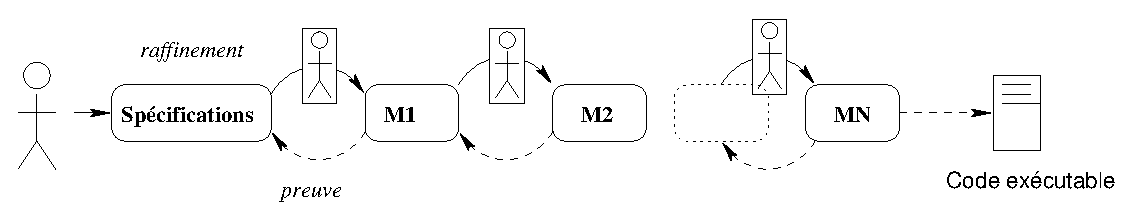
\epsfig{width=.8\textwidth, file=figures/fig-process-b.eps}
    \caption{D\'eveloppement formel par raffinement}
    \label{fig-process-b}
\end{figure}

Cette m\'ethode pr\'esente l'avantage \'evident de produire une application
dont la validit\'e eu \'egard aux sp\'ecifications est
\emph{prouv\'ee}, sous r\'eserve de la preuve de correction de la
projection terminale d'un mod\`ele en code. 

Une autre solution est, toujours \`a partir d'une expression formelle des
exigences, de produire automatiquement des \emph{cas de test} qui
permettront \`a l'issue du processus de d\'eveloppement  de valider
le logiciel produit : c'est ce qu'illustre la figure
\ref{fig-process-test}. 

\begin{floatingfigure}{.5\textwidth}
    \centering
    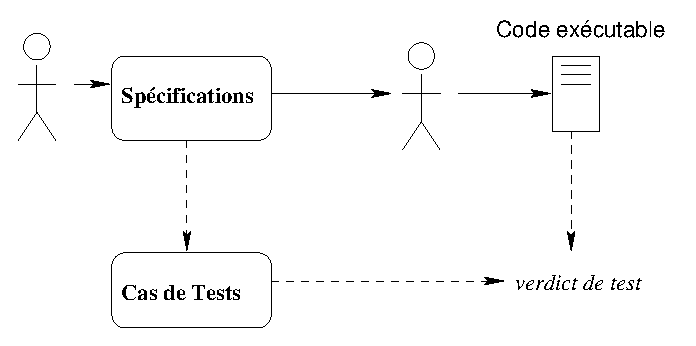
\epsfig{width=.45\textwidth, file=figures/fig-process-test.eps}
    \caption{D\'eveloppement formel par test}
    \label{fig-process-test}
\end{floatingfigure}

La premi\`ere solution est aujourd'hui inaccessible dans le contexte
qui est le notre, pour un certain nombre de raisons : le niveau de
fiabilit\'e exig\'e dans les applications de syst\`emes
d'informations est nettement moins \'elev\'e que dans des
syst\`emes critiques temps r\'eels ; le co\^ut de la mise en \oe
uvre de m\'ethodes formelles est tr\`es \'elev\'e, surtout compte
tenu du fait que la phase de preuve ne peut \^etre en l'\'etat
actuel des m\'ethodes et outils totalement automatis\'ee ;
l'int\'er\^et de mettre en place un tel processus dans des
syst\`emes h\'et\'erog\`enes en constante \'evolution para\^{\i}t
limit\'e. 

La seconde solution para\^{\i}t plus ais\'ee \`a mettre en place. Elle
exige toutefois un certain nombre de pr\'e-requis : l'existence d'une
sp\'ecification suffisamment formalis\'ee pour permettre la
d\'erivation automatique de cas de tests pertinents ; le maintien
d'une coh\'erence dans le processus de d\'eveloppement permettant de
faire en sorte que les cas de tests produits initialement restent
applicable \`a l'autre bout de la cha\^{\i}ne, c'est \`a dire lors de
la construction du logiciel fini ; l'existence de proc\'edures
automatiques fiables et de mesures de la fiabilit\'e atteinte par
l'ex\'ecution d'un ensemble donn\'e de tests. 

Le but de ce travail est donc de faire en sorte que ces deux solutions
au probl\`eme de la qualit\'e des logiciels produits : un processus
de d\'eveloppement centr\'e sur une architecture de composants
hi\'erarchiques, un processus de test automatis\'e et fiable, se
rejoignent.

%%% Local Variables: 
%%% mode: latex
%%% TeX-master: "these"
%%% TeX-master: "these"
%%% TeX-master: "these"
%%% End: 
    